\documentclass[11pt, addpoints]{exam}

\bibliographystyle{abbrv}

\usepackage{amsfonts}

\usepackage{amsthm}

\usepackage{amssymb}

\usepackage{amsmath}

\usepackage{enumerate}

\usepackage[all]{xy}

\usepackage{graphicx}

\usepackage{tikz}

\usepackage{pgfplots}
\usepgfplotslibrary{fillbetween}
\usetikzlibrary{arrows}

\newcommand{\N}{\mathbb{N}}

\newcommand{\Z}{\mathbb{Z}}

\newcommand{\R}{\mathbb{R}}

\newcommand{\Q}{\mathbb{Q}}

\newcommand{\C}{\mathbb{C}}

\newcommand{\T}{\mathbb{T}}

\newcommand{\ra}{~~\Rightarrow~~}

\newcommand{\lra}{~~\Leftrightarrow~~}

\setlength{\unitlength}{1.5cm}

\addpoints

\begin{document}




\section*{Math 241 Summer 2023 Final Study Guide}

\textbf{Name:}

\begin{flushright}
\gradetable[v][questions]
\end{flushright}     

\begin{itemize}
\item You may not use calculators on the test.  
\item You may use \textbf{paper} notes on the test.
\item Please ask if anything seems confusing or ambiguous.
\item You must show all your work and make clear what your final solution is (e.g.\ by drawing a box around it).
\item Good luck!
\end{itemize}

           

\pagebreak

[This page is intentionally left almost blank.]

\pagebreak

\begin{questions}

\question[40] Sketch the curve $f(x)$ given by
\[f(x) = \frac{(x-1)^2}{2x^2}.\]
Find the following values exactly:
\begin{itemize}
    \item Roots of $f$.
    \item Vertical and horizontal asymptotes of $f$.
    \item Intervals of increase and decrease.
    \item Absolute minimums and absolute maximums, if they exist.
    \item Local minimums and local maximums, if they exist.
    \item Intervals of concavity.
    \item Inflection points, if they exist.
\end{itemize}

\begin{align*}
    f(x) & = \frac{x^2-2x+1}{2x^2} = \frac{1}{2} - \frac{1}{x} + \frac{1}{2x^2}\\
    f'(x) & = \frac{1}{x^2} - \frac{1}{x^3} = \frac{x-1}{x^3} \\
    f''(x) & = -\frac{2}{x^3} + \frac{3}{x^4} = \frac{3-2x}{x^4}
\end{align*}

The roots are $x=1$. The horizontal asymptote is $y = \frac{1}{2}$. The vertical asymptotes are $x=0$.
\begin{center}
\begin{tikzpicture}
    \begin{axis}[
        axis y line=none,
        axis lines=left,
        axis line style={-},
        xmin=-3,
        xmax=3,
        xtick={-3,...,3},
        ymin=0,
        ymax=1,
        xlabel=$f(x)$,
        scatter/classes={o={mark=*}},
        restrict y to domain=0:1,
        width = 5.5in,
        height = 1in,
        ]
        \addplot table [only marks, y expr=0, meta index=1, header=false] {
        1 o
        0 o
        };
        % \node[coordinate,label=above:{$x=0$}] at (axis cs:0,0.05) {};
        % \node[coordinate,label=above:{$x=1$}] at (axis cs:1,0.05) {};
        \node[coordinate, label = above:{$+$}] at (axis cs:-1.5,0.05) {};
        \node[coordinate, label = above:{$+$}] at (axis cs:0.5,0.05) {};
        \node[coordinate, label = above:{$+$}] at (axis cs:2,0.05) {};
    \end{axis}
\end{tikzpicture}  
\end{center}
The critical points are $x=0,1$.
\begin{center}
\begin{tikzpicture}
    \begin{axis}[
        axis y line=none,
        axis lines=left,
        axis line style={-},
        xmin=-3,
        xmax=3,
        xtick={-3,...,3},
        ymin=0,
        ymax=1,
        xlabel=$f'(x)$,
        scatter/classes={o={mark=*}},
        restrict y to domain=0:1,
        width = 5.5in,
        height = 1in,
        ]
        \addplot table [only marks, y expr=0, meta index=1, header=false] {
        0 o
        1 o
        };
        % \node[coordinate,label=above:{$x=0$}] at (axis cs:0,0.05) {};
        % \node[coordinate,label=above:{$x=1$}] at (axis cs:1,0.05) {};
        \node[coordinate, label = above:{$+$}] at (axis cs:-1.5,0.05) {};
        \node[coordinate, label = above:{$-$}] at (axis cs:0.5,0.05) {};
        \node[coordinate, label = above:{$+$}] at (axis cs:2,0.05) {};
    \end{axis}
\end{tikzpicture}  
\end{center}
By the above graph, $x=1$ is a local minimum. $x=0$ is not a local maximum because it is a vertical asymptote. Using this information, the absolute minimum is $f(1) = 0$. The absolute maximum does not exist since the vertical asymptote goes up to infinity.

The inflection points are $x = 0, \frac{3}{2}$.
\begin{center}
\begin{tikzpicture}
    \begin{axis}[
        axis y line=none,
        axis lines=left,
        axis line style={-},
        xmin=-3,
        xmax=3,
        xtick={-3,...,3},
        ymin=0,
        ymax=1,
        xlabel=$f''(x)$,
        scatter/classes={o={mark=*}},
        restrict y to domain=0:1,
        width = 5.5in,
        height = 1in,
        ]
        \addplot table [only marks, y expr=0, meta index=1, header=false] {
        0 o
        1.5 o
        };
        % \node[coordinate,label=above:{$x=0$}] at (axis cs:0,0.05) {};
        % \node[coordinate,label=above:{$x=1$}] at (axis cs:1,0.05) {};
        \node[coordinate, label = above:{$+$}] at (axis cs:-1.5,0.05) {};
        \node[coordinate, label = above:{$+$}] at (axis cs:0.75,0.05) {};
        \node[coordinate, label = above:{$-$}] at (axis cs:2.25,0.05) {};
    \end{axis}
\end{tikzpicture}  
\end{center}

\pagebreak
Putting it all together, we obtain the graph below.
\vfill
\begin{center}
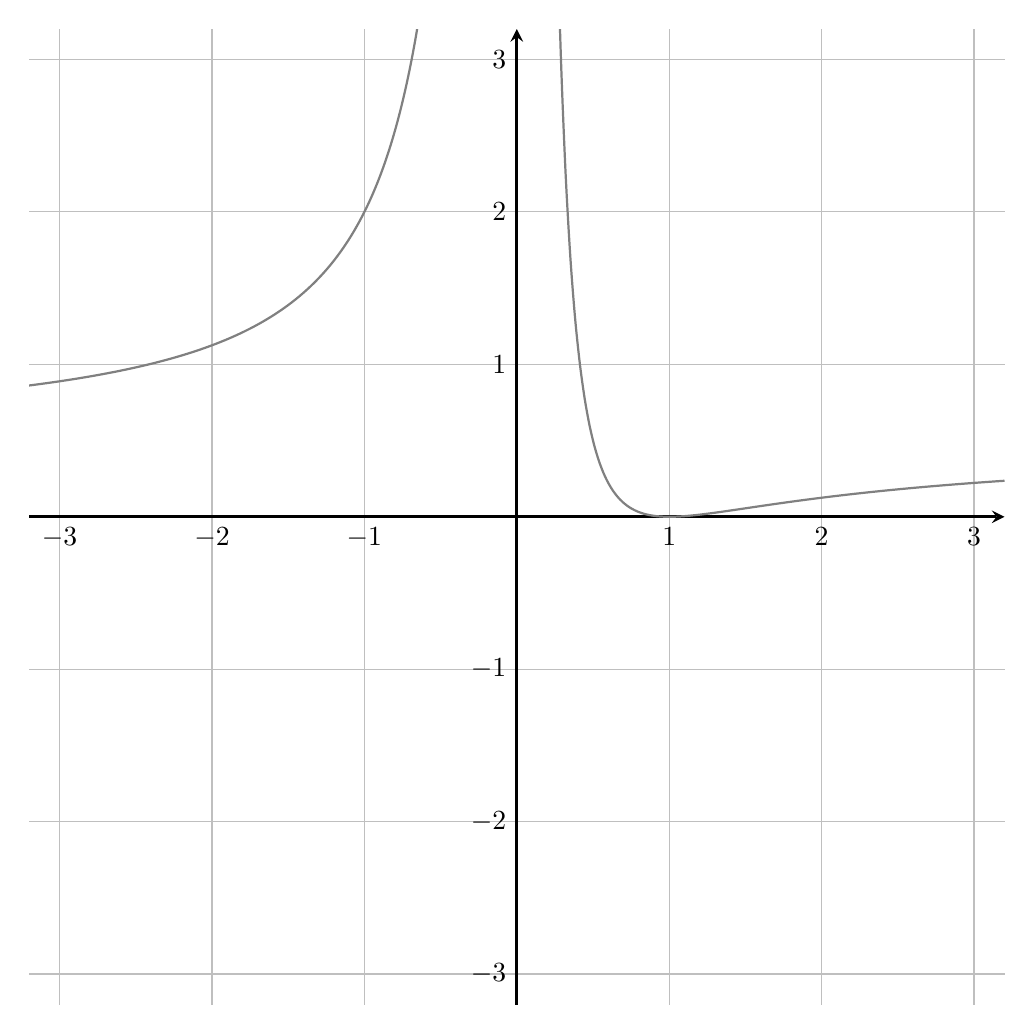
\begin{tikzpicture}
\begin{axis}[thick,smooth,no markers,
        xmin=-3.2, xmax=3.2,
        ymin=-3.2, ymax=3.2,
        xtick={-3,...,3},  
        % xticklabels= {,,},
        ytick={-3,...,3},
        % yticklabels= {,,},
        major tick length={0},
        line width=1pt,
        axis lines=center, height=5.5in, width = 5.5in, grid=major]
        \addplot [domain=-3.2:-0.1, samples=100, name path=f, thick, color=black!50]
        {((x-1)^2)/(2*x^2)} ;
        \addplot [domain=0.1:3.2, samples=100, name path=f, thick, color=black!50]
        {((x-1)^2)/(2*x^2)} ;
\end{axis}
\end{tikzpicture}
\vspace{1.5in}
\end{center}

\pagebreak

\question $\ $

\begin{parts}
    \part[10]
    Show that the equation $8x + 4\sin{x} + 6 = 0$ has a root.

    Let $f(x) := 8x+4\sin{x} + 6$. Then $f(0) = 6 > 0$ and $f(-10\pi) = -80\pi +6 < 0$. Since $f(x)$ is continuous on the interval $[-10\pi,0]$ and $f(-10\pi) < 0 < f(0)$, then by the \textbf{Intermediate Value Theorem}, there must exist a point $c$ in the range $(-10\pi, 0)$ such that $f(c) = 0$. 
    \vfill
    \part
    (7 points \textbf{EXTRA CREDIT}) Show that the above equation has exactly one root.
    
    Suppose for contradiction that $f$ has another root $d \neq c$. Then $f(d) = 0$. Since $f$ is continuous and differentiable on the range $(c,d)$ (or $(d,c)$), whatever makes sense), then \textbf{Mean Value Theorem} applies, and thus there is a value $x=e$ such that $f'(e) = \frac{f(d)-f(x)}{d-c} = \frac{0}{d-c} = 0$. But $f'(x) = 8 + 4\cos{x} \geq 8-4 = 4$. Since $f'(x) > 0$ for any $x$ on the real number line, then $f'(e) \neq 0$. Therefore, a contradiction has been obtained and thus another root can not have existed.
    \vfill
\end{parts}

\pagebreak

\question[10] Find the point on the curve $y = \sqrt{x}$ that is closest to the point $(3,0)$.

Let $d(x)$ be the distance function from the curve to $(3,0)$. Then
\[d(x) = \sqrt{(x-3)^2 + y^2} = \sqrt{(x-3)^2 + x}.\]
Taking the derivative, we find that
\[d'(x) = \frac{2x-5}{2d}\]
so the critical point is $x=5/2$. This turns out to be a minimum, and thus $(5/2,\sqrt{5/2})$ is the closest point to $(3,0)$.
\vfill

\pagebreak

\question[10] Evaluate the following
\[\frac{d}{dx} \int_{x^3}^{-5318008} \sec^7(t^3) + t \ dt.\]
\begin{align*}
    \frac{d}{dx} \int_{x^3}^{-5318008} \sec^7(t^3) + t \ dt & = \frac{d}{dx} \left(-\int^{x^3}_{-5318008} \sec^7(t^3) + t \ dt \right) = -\left(\sec^7(x^9) + x^3\right) \cdot 3x^2
\end{align*}
\vfill
\question Evaluate the following definite integrals, if they exist.
\begin{parts}
    \part[10] $\displaystyle \int_1^5 \frac{2t}{(t^2+4)^2} \ dt$
    \begin{align*}
        u = t^2 + 4 & \quad du = 2t \ dt \\
        \int_1^5 \frac{2t}{(t^2+4)^2} \ dt & = \int_5^{29} u^{-2} \ du = \left[-\frac{1}{u}\right]_5^{29} \\
        & = \frac{1}{5} - \frac{1}{29}
    \end{align*}
    \vfill
    \pagebreak
    \part[10] $\displaystyle \int_0^{\pi/4} (1+\cos{\theta})^3 \sin{\theta} \ d\theta$
    \begin{align*}
        u = 1+\cos{\theta} & \quad du = -\sin{\theta} d\theta \\
        \int_0^{\pi/4} (1+\cos{\theta})^3 \sin{\theta} \ d\theta & = \int_2^{1+\sqrt{2}/2} -(1+u)^3 \ du \\
        v = 1 + u & \quad dv = du \\
        & = \int_3^{2+\sqrt{2}/2} -v^3 \ dv = -\frac{1}{4}[v^4]_3^{2+\sqrt{2}/2} \\
        & = -\frac{1}{4}\left(\left(2+\frac{\sqrt{2}}{2}\right)^4 - 3^4\right)
    \end{align*}
    \vfill
    \part[10] $\displaystyle \int_{-\pi/4}^{\pi/4} x^3 \cos^2{x} \ dx$

    $x^3$ is odd and $\cos^2{x}$ is even. Therefore, the integrand is odd. The integral is 0.
    \vfill
\end{parts}

\pagebreak

\question[20] Find the volume of a solid obtained by rotating the region bounded by the given curve about the specified axis.
\begin{align*}
    & y = 2x \\
    & y = x^2\\
    & \text{About the $x$-axis}
\end{align*}

\begin{center}
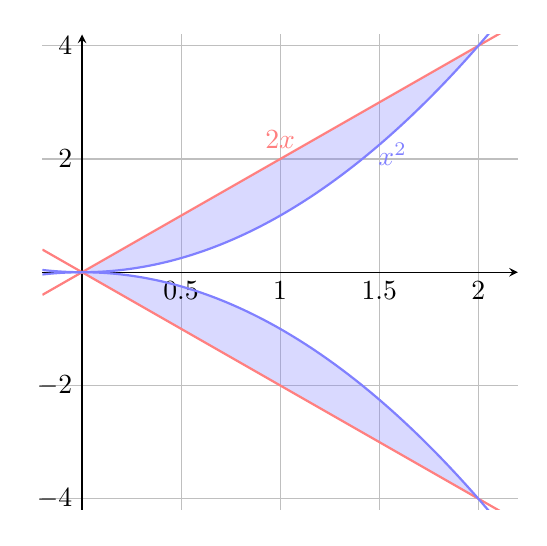
\begin{tikzpicture}
\begin{axis}[thick,smooth,no markers,
        xmin=-0.2, xmax=2.2,
        ymin=-4.2, ymax=4.2,
        % xtick={-4,...,4},  
        % xticklabels= {,,},
        % ytick={-4,...,4},
        % yticklabels= {,,},
        major tick length={0},
        line width=1pt,
        axis lines=center, height=3in, width = 3in, grid=major]
        \addplot [domain=-0.2:2.2, samples=100, name path=f, thick, color=red!50]
        {2*x} node[above,pos=0.5] {$2x$} ;
        \addplot [domain=-0.2:2.2, samples=100, name path=g, thick, color=blue!50]
        {x^2} node[right,pos=0.5] {$x^2$} ;
        \addplot[blue!50, opacity=0.3] fill between[of= f and g, soft clip={domain=0:2}];
        \addplot [domain=-0.2:2.2, samples=100, name path=h, thick, color=red!50]
        {-2*x} ;
        \addplot [domain=-0.2:2.2, samples=100, name path=i, thick, color=blue!50]
        {-x^2} ;
        \addplot[blue!50, opacity=0.3] fill between[of= h and i, soft clip={domain=0:2}];
\end{axis}
\end{tikzpicture}
\end{center}

This volume can be calculated using cross sectional areas. The volume is
\begin{align*}
    \int_0^2 A(x) \ dx & = \int_0^2 \pi (2x)^2 - \pi (x^2)^2 \ dx\\
    & = \pi \int_0^2 4x^2 - x^4 \ dx \\
    & = \pi\left[\frac{4}{3} x^3 - \frac{1}{5}x^5\right]_0^2 \\
    & = \pi\left(\frac{4}{3}2^3 - \frac{1}{5}2^5\right)
\end{align*}
\end{questions}
    
\end{document}
